% ! TeX root = ../../thesis.tex
\chapter{Analisi e Progettazione}
\label{chapter:analysis}
In questo secondo capitolo viene presentata l'analisi dei requisiti e il \textit{design} del sistema.
%
Nei primi due paragrafi vengono elencati i requisiti del sistema ed è descritto il dominio applicativo.
%
Il terzo paragrafo è dedicato al \textit{design} dell'applicativo: si parte da una visione architetturale e a seguire si dettagliano le parti di \textit{design} più rilevanti al fine di chiarificare la logica con cui è stato implementato il sistema.

\section{Requisiti}
Come già anticipato, lo scopo della tesi è realizzare un sistema antiplagio automatico in grado d'individuare eventuali porzioni di codice copiato nei progetti \textit{software} del corso di Programmazione ad Oggetti dell'Università di Bologna.

Di seguito vengono descritti, per punti, i requisiti del sistema, suddivisi tra requisiti \textit{funzionali} e \textit{non funzionali}.

\subsection*{Requisiti funzionali}
\begin{itemize}
    \item Il sistema riceve in \textit{input} un insieme di progetti di cui si vuole verificare l'autenticità, detto \textbf{\textit{Submission}}, e un insieme di progetti con cui confrontarli, detto \textbf{\textit{Corpus}};
    
    \item Il confronto viene effettuato tra progetti sviluppati nello stesso linguaggio di programmazione.
    
    \item I progetti sono sviluppati in linguaggio Java e mantenuti in \textit{repository} pubbliche su \textit{GitHub} e \textit{Bitbucket}\footnote{
        \href{https://github.com}{\textit{GitHub}} e \href{https://bitbucket.org}{\textit{Bitbucket}} sono due tra i più conosciuti servizi di \textit{hosting} per progetti \textit{software} che utilizzano sistemi di controllo di versione decentralizzati, come \href{https://git-scm.com}{Git}.
    }. Si assume che i progetti passati siano tempo-invarianti: dal momento in cui vengono corretti, le rispettive \textit{repository} sono archiviate e mai più modificate;

    \item Il sistema deve fornire in \textit{output} le sezioni di codice che, con un determinato livello di accuratezza, ha stabilito essere simili.
\end{itemize}

\subsection*{Requisiti non funzionali}
\begin{itemize}
    \item L'algoritmo per determinare la similarità, così come le metriche utilizzate, devono essere interscambiabili e facilmente estendibili;
    \item Le informazioni estrapolate dai sorgenti sono salavate in modo tale da essere riutilizzate nelle analisi successive di altri progetti;
    \item \`E necessario che il sistema impieghi un tempo "ragionevole" per effettuare la computazione;
\end{itemize}

\section{Analisi e modello del dominio}
% descrizione session?
Il sistema deve essere in grado, a partire da un insieme di \textit{repository}, corrispondenti a progetti coerenti per linguaggio di programmazione, di estrarne una rappresentazione confrontabile (\textit{SourceRepresentation}) medianti opportuni algoritmi di analisi (\textit{Analyzer}).
%
Ciascuna coppia di rappresentazioni intermedie deve essere successivamente confrontata da algoritmi di rilevamento di somiglianze (\textit{PlagiarismDetector}) al fine di poter determinare eventuali parti di codice duplicato e/o somiglianze, generando infine dei \textit{report}.

Gli elementi costitutivi il problema sono sintetizzati in \Cref{img:02-domain}.

La principale difficoltà sarà individuare tecniche di analisi e di rilevamento delle somiglianze che siano robuste, ovvero permettano d'identificare casi dii copiature anche se lo sviluppatore ha effettuato modifiche per oscurarle.
%
Particolare attenzione dovrà essere posta sulla progettazione dei componenti per l'analisi e per il confronto, in quanto, data la natura del sistema, possono dover cambiare frequentemente ed essere fortemente configurabili.
%
Inoltre, il requisito non funzionale sulle \textit{performance} richiederà un'analisi dei tempi di esecuzione non appena il sistema sarà completato.

\begin{figure}[h!]
    \centering
    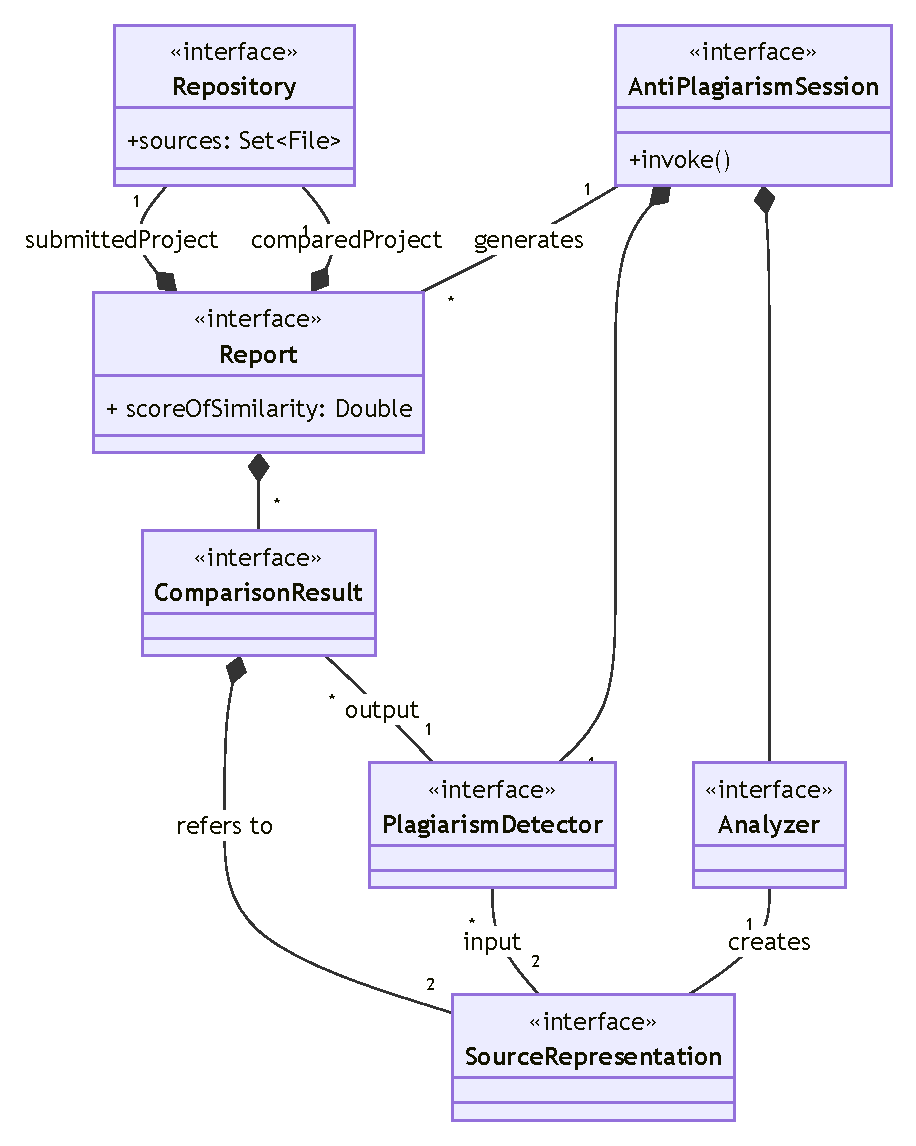
\includegraphics[width=0.8\textwidth]{resources/img/02-domain.pdf}
    \caption{Schema UML delle classi dell'analisi del problema, con rappresentate le entità principali ed i rapporti fra loro.}
    \label{img:02-domain}
\end{figure}

\section{\textit{Design}}

\subsection{Architettura}
% manca la trattazione degli input...
L'architettura del sistema è così organizzata: \textbf{\textit{AntiPlagiarismSession}} è l'interfaccia responsabile della logica dell'applicazione e rappresenta una specifica sessione, dove per sessione si intende l'entità che, una volta opportunamente configurata con gli opportuni analizzatori, \textit{provider} di progetti e \textit{output}, esegue la logica dell'applicazione.

Gli \textbf{\textit{Output}} rappresentano le risorse su cui andare a rappresentare i risultati ottenuti, mentre il \textbf{\textit{RepositoryProvider}} rappresenta la strategia con cui recuperare i progetti su cui effettuare l'analisi.

Il confronto e l'analisi dei sorgenti vengono effettuati, rispettivamente, dal \textbf{\textit{PlagiarismDetector}} e dall'\textbf{\textit{Analyzer}}, che incapsula la specifica strategia utilizzata e demanda a \textbf{\textit{KnoledgeBaseRepository}} il salvataggio e il recupero delle rappresentazioni dei sorgenti già precedentemente analizzati e, perciò, salvati.

Questa architettura permetterebbe facilmente l'aggiunta di un nuovo \textbf{\textit{Output}} e di poter cambiare sia la strategia per recuperare i progetti, sia la logica con cui questi vengono processati.

In \Cref{img:02-architecture} è esemplificato il diagramma UML architetturale.

\begin{figure}[h!]
    \centering
    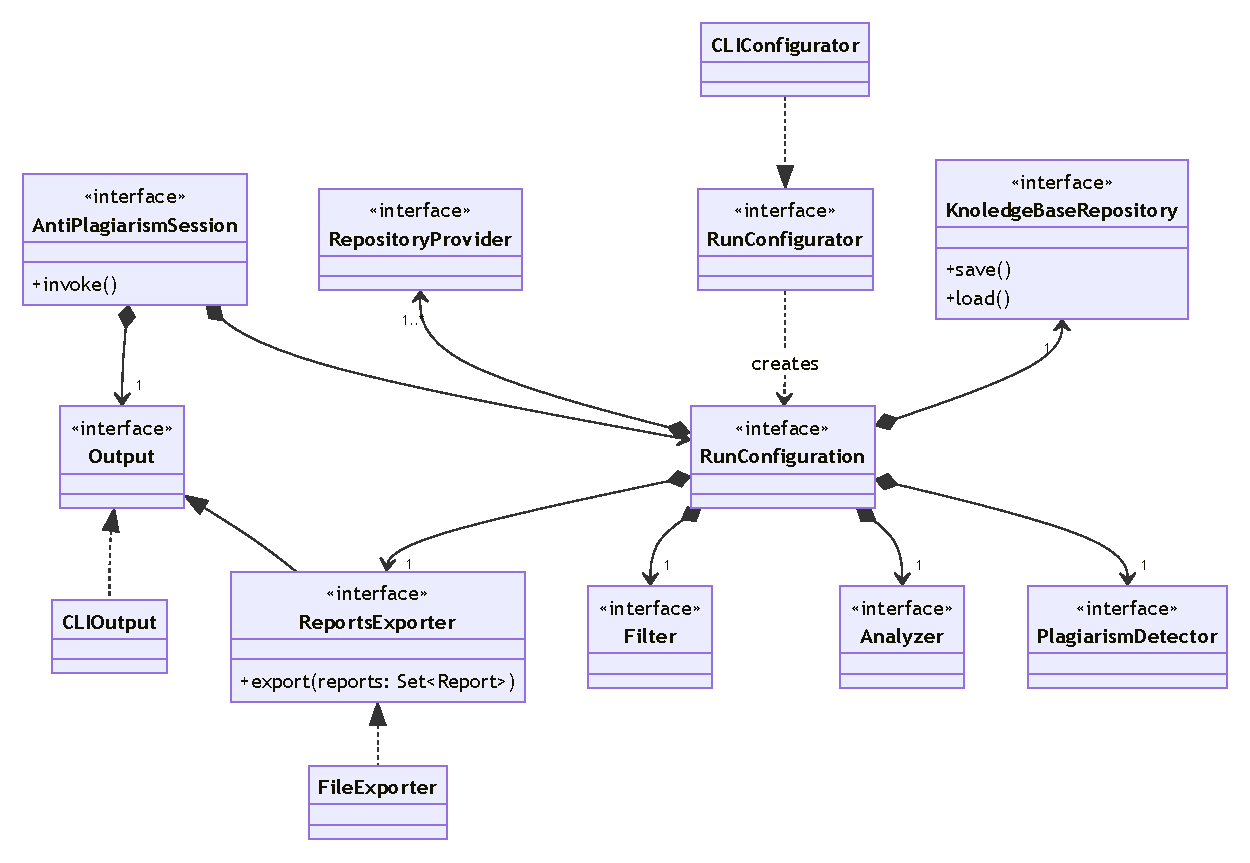
\includegraphics[width=\textwidth]{resources/img/02-achitecture.pdf}
    \caption{Schema UML architetturale del sistema.}
    \label{img:02-architecture}
\end{figure}

\subsection{\textit{Design} dettagliato}
In questa sezione si presenta in modo dettagliato le singole componenti del sistema.

\subsubsection*{\textit{Provider} dei progetti}
Per quanto concerne i \textit{provider} di \textit{repository}, ovvero i componenti che devono recuperare i sorgenti dei progetti da \textit{repository} pubbliche da \textit{GitHub} e/o da \textit{Bitbucket}, si è scelto un \textit{design} che permettesse il massimo riuso degli elementi comuni, aderendo a uno schema interfaccia - classe astratta - classe concreta.

In \Cref{img:02-provider} è riportato lo schema UML delle classi dei \textit{provider}.

\begin{figure}[h!]
    \centering
    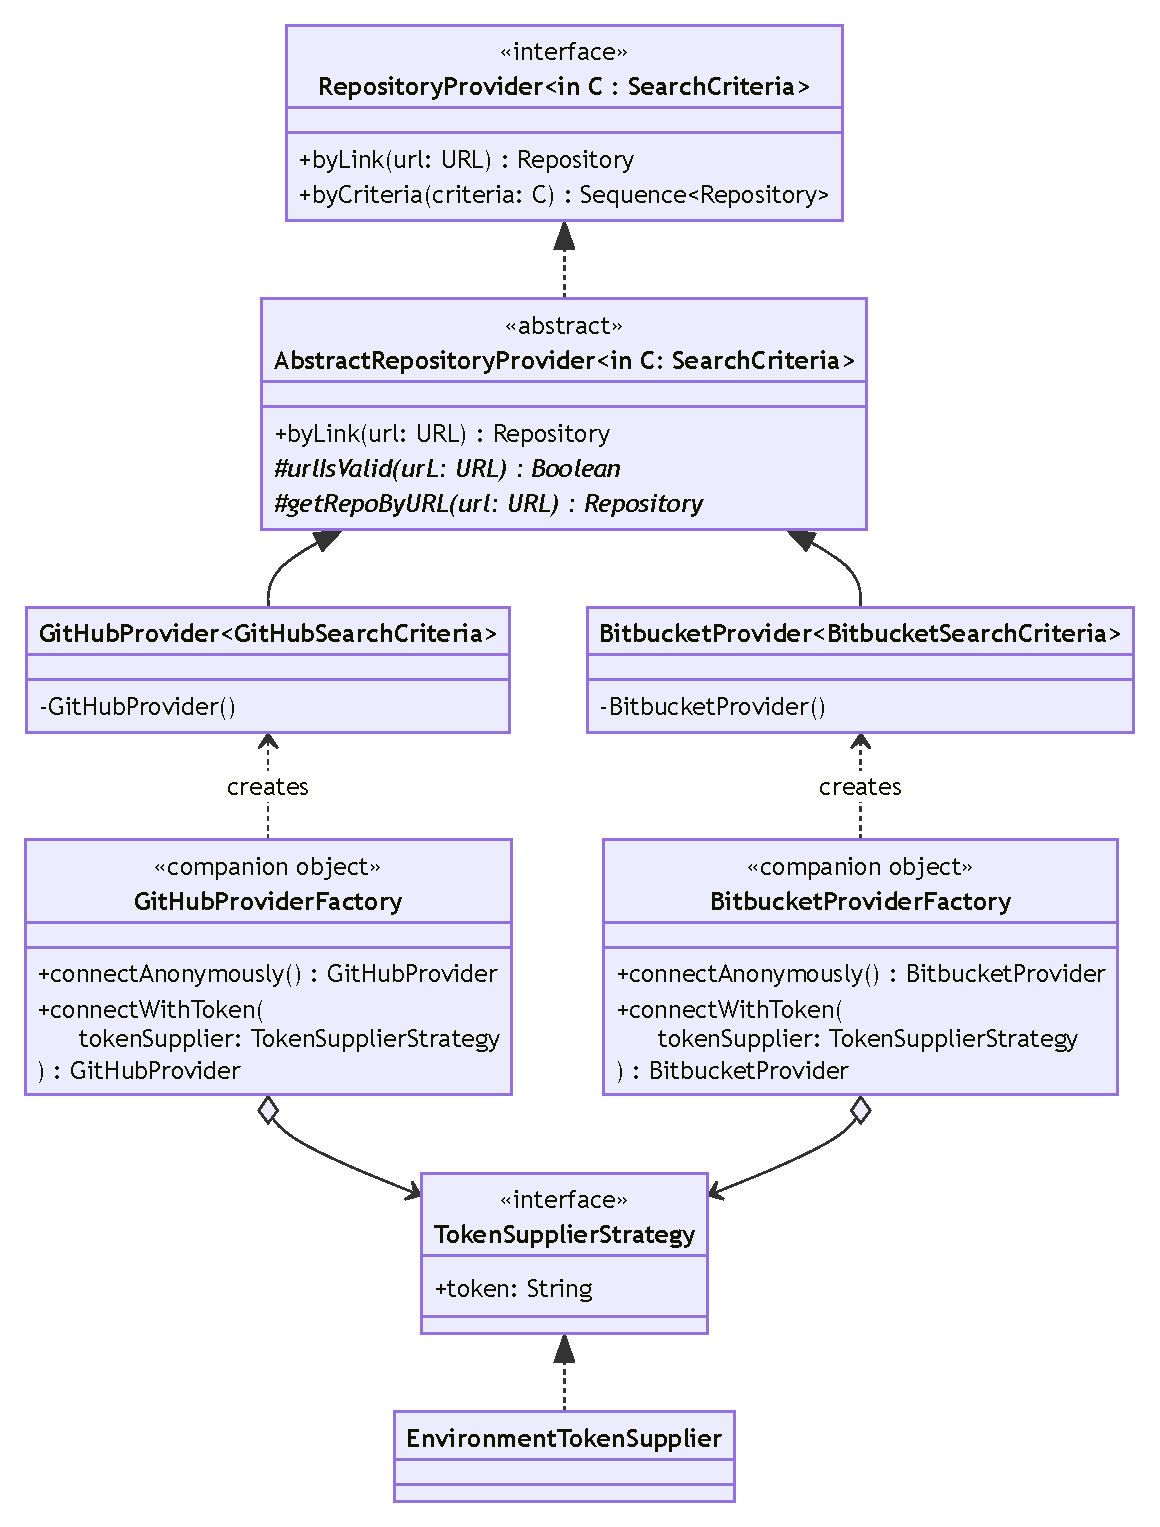
\includegraphics[width=0.9\textwidth]{resources/img/02-provider.pdf}
    \caption{Schema UML dei provider.}
    \label{img:02-provider}
\end{figure}

Viste le limitazioni in termini di richieste che i due servizi espongono e la conseguente necessità di autenticarsi mediante degli opportuni \textit{token} per effettuare le richieste \textit{REST}, si è optato di demandare la logica di recupero dei suddetti \textit{token} di autenticazione all'interfaccia \textit{TokenSupplierStrategy} che fa da \textit{Strategy}.
%
% quali limiti? nota a piè di pagina :)
%
L'implementazione di default ricerca tra variabili d'ambiente, ma questo approccio può essere facilmente esteso.
%
% devo descrivere cosa fa strategy? magari una nota a piè di pagina...
%
La creazione dei provider avviene per mezzo di due \textit{static factory}, incapsulate all'interno dei due \textit{provider}, in modo da permettere di ottenere un oggetto \textit{provider} anche senza autenticazione.
%
Nonostante questo sia in genere sconsigliato per via delle limitazioni sopra citate, può essere utile in fase di \textit{testing} e per permettere di testare il sistema anche con la CI attiva, in contesti in cui non sia possibile usare i veri \textit{token} di autenticazione.
% consider static factory effective kotlin
% riferimento alla CI

Dopo una prima analisi delle \textit{API} dei due servizi di \textit{hosting} si è convenuto di permettere di recuperare i progetti mediante due metodi: un \textit{link} diretto alla \textit{repository}, oppure mediante un criterio di ricerca, rappresentato dall'interfaccia \textit{SearchCriteria}.
%
Per permettere che questi siano componibili è stato qui utilizzato il pattern \textit{Decorator}.
%
In questo modo possono essere creati dinamicamente criteri compositi in base alle esigenze e in futuro potrebbero essere aggiunti nuovi criteri di ricerca, come il fatto di essere archiviate o il numero di stelle che ha ricevuto un determinato progetto.
%
Il \textit{design} è presentato in \Cref{img:02-search-criteria}.

\begin{figure}[h!]
    \centering
    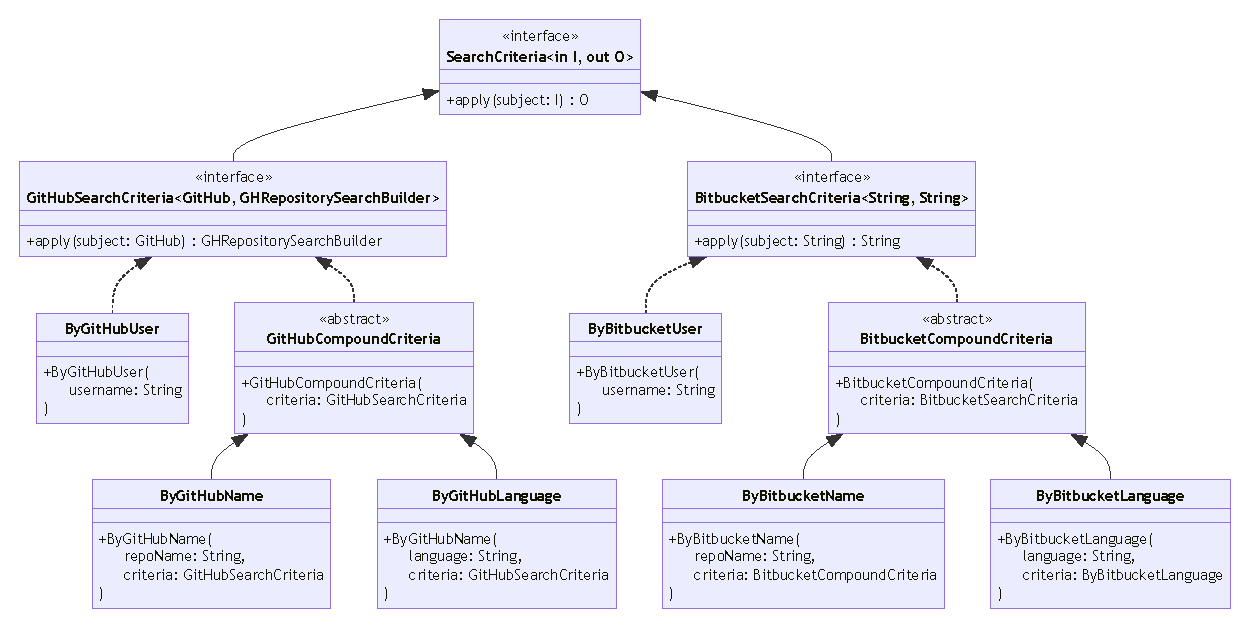
\includegraphics[width=\textwidth]{resources/img/02-search-criteria.pdf}
    \caption{Schema UML dei criteri di ricerca delle \textit{repository}.}
    \label{img:02-search-criteria}
\end{figure}

% inserire repository

\subsubsection*{Analizzatore e \textit{detector}}
L'analizzatore e il \textit{detector} sono il cuore dell'intero sistema.
%
Il loro \textit{design} è stato pensato in modo tale che permettesse il massimo grado di configurabilità e di estendibilità.
%
Presumibilmente, infatti, questi sono i componenti che varieranno più spesso nell'arco del ciclo di vita di questo \textit{software} e il cui grado di configurabilità influirà certamentente in modo preponderante sia sulle prestazioni, sia sull'efficacia del sistema.

L'analizzatore è il componente che si occupa di trasformare i file sorgenti in rappresentazioni confrontabili.
%
Indipendentemente dalla tipologia di analisi che si voglia applicare, la trasformazione non avviene tramite un semplice passaggio, bensì una sequenza di operazioni che sono eseguite sequenzialmente in cascata.
%
Calato nella specifica strategia utilizzata per l'implementazione dello strumento, queste sono: il \textit{parsing} del file, una fase di \textit{preprocessing} ed infine la \textit{tokenizzazione} del sorgente.
%
Questa sequenza di azioni è naturalmente modellata attraverso il pattern \textit{Pipeline}: ogni singolo stadio della \textit{pipeline} è modellato attraverso l'interfaccia \texttt{StepHandler}; la sequenza di \textit{handler} viene poi costruita all'interno del concreto \texttt{Analyzer}, nel nostro caso \texttt{JavaTokenizationAnalyzer}.
%
% manca tokenTypeSupplier
% ref pipeline pattern?
%

\begin{figure}[h!]
    \centering
    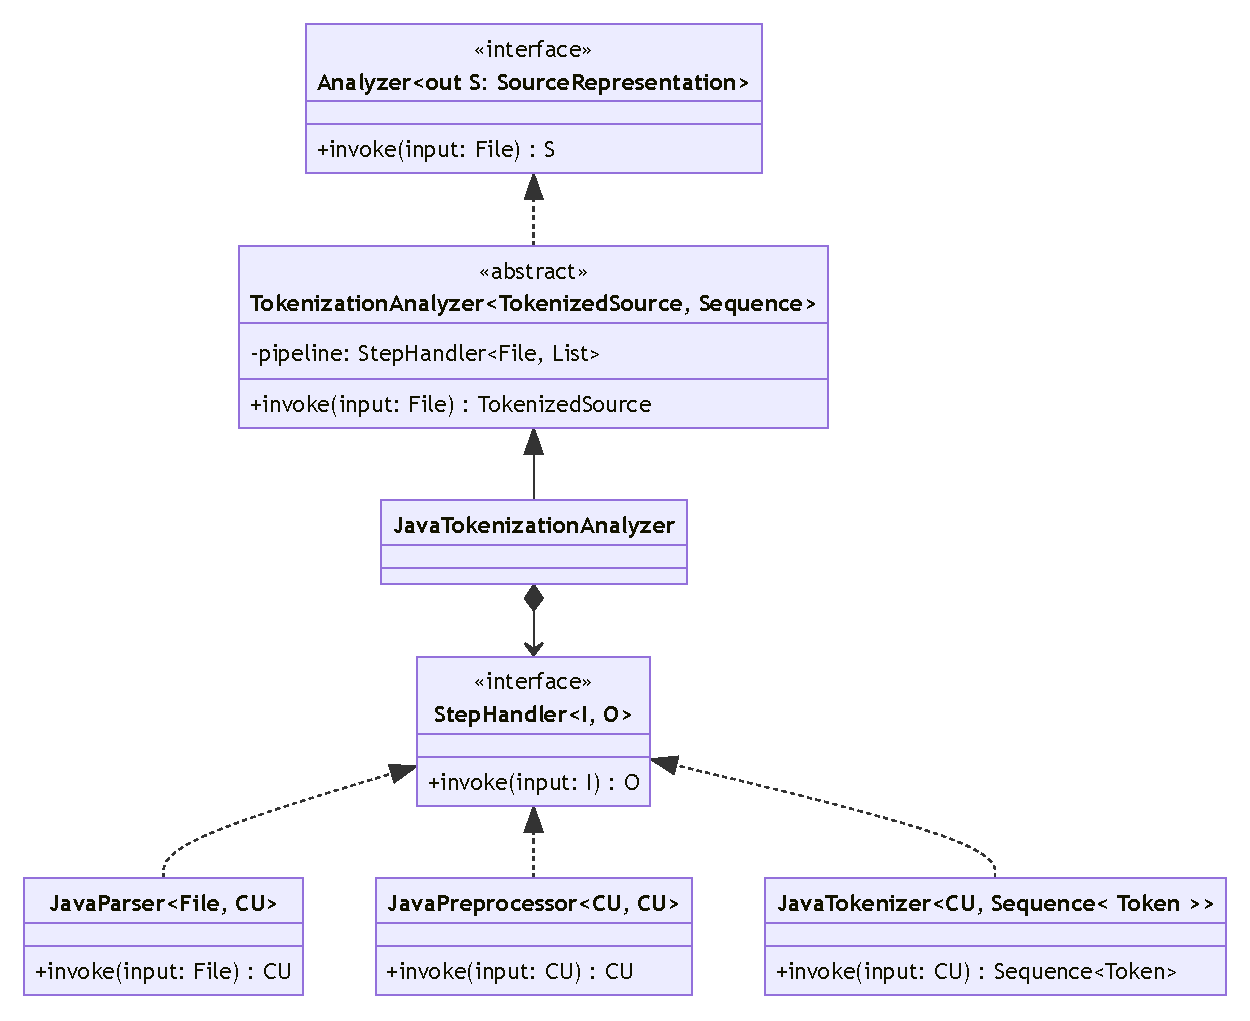
\includegraphics[width=\textwidth]{resources/img/02-analyzer.pdf}
    \caption{Schema UML dell'analizzatore.}
    \label{img:02-analyzer}
\end{figure}

La rappresentazione intermedia prodotta dall'analizzatore è modellata dall'interfaccia \texttt{SourceRepresentation}. 
%
Tra tutte, quella implementata nell'attuale sistema è composta da sequenza di \textit{token} e perciò denominata \texttt{TokenizedSource}.

L'elenco dei possibili tipi di \textit{token} dipende chiaramente dal linguaggio utilizzato.
%
La strategia di recupero di questi ultimi è affidata, al solito tramite \textit{Strategy}, a \texttt{TokenTypesSupplier}.

\begin{figure}[h!]
    \centering
    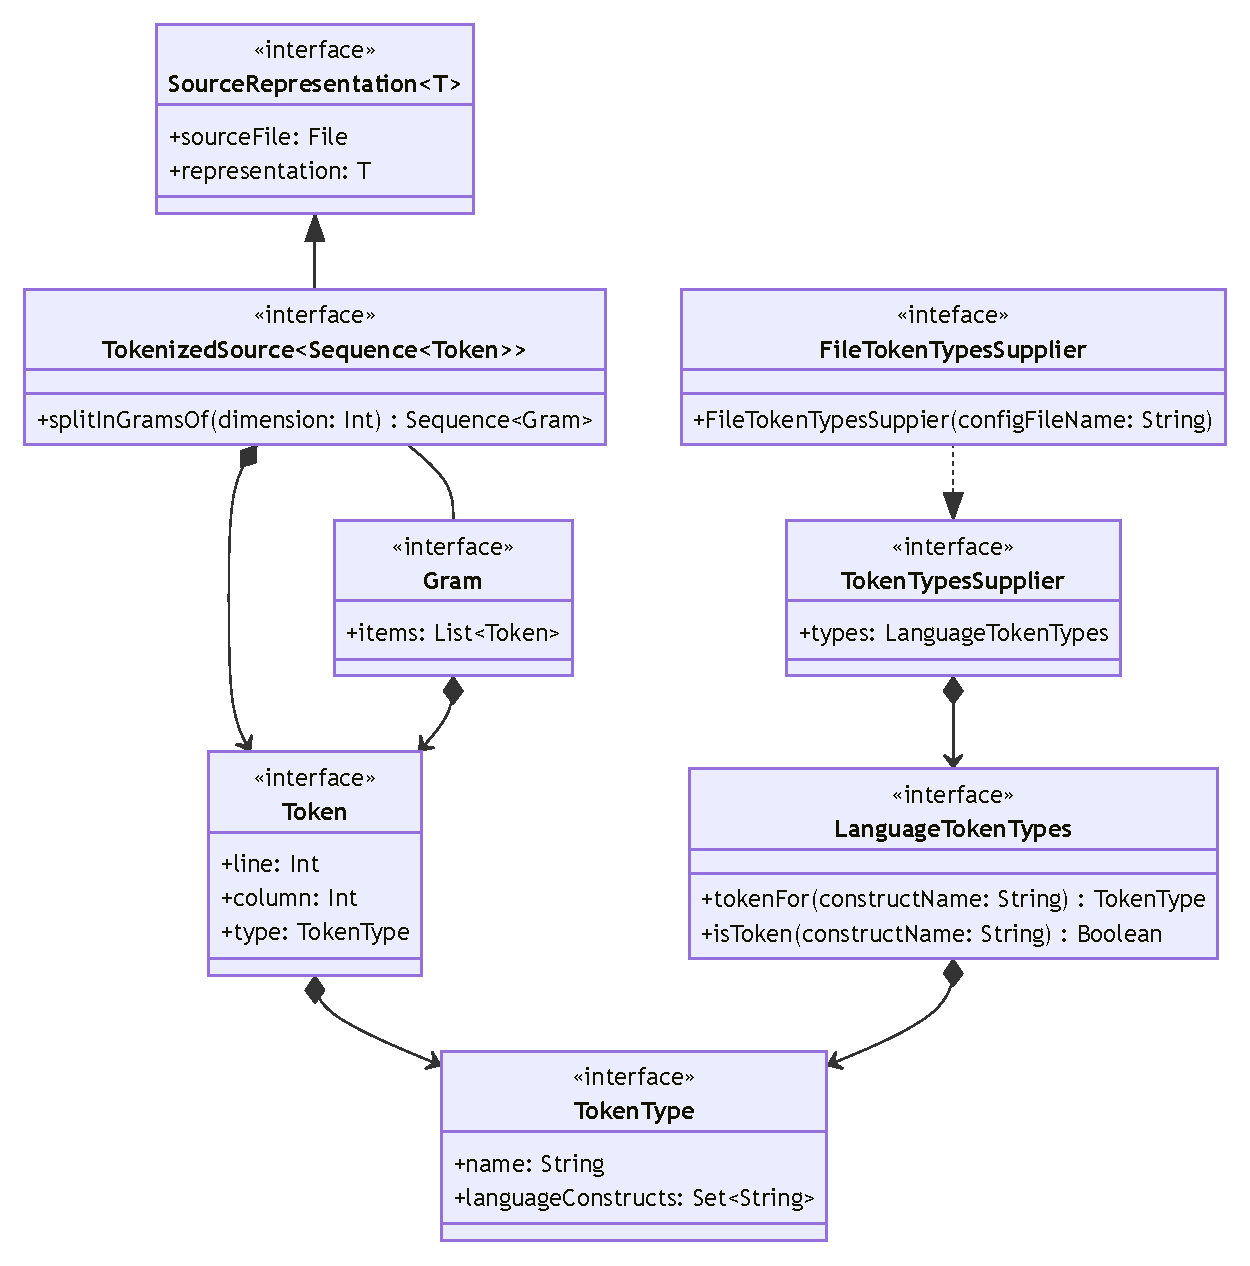
\includegraphics[width=\textwidth]{resources/img/02-representations.pdf}
    \caption{Schema UML delle rappresentazioni intermedie.}
    \label{img:02-representations}
\end{figure}

\texttt{PlagiarismDetector} rappresenta invece il componente che individua le similarità tra una coppia di \texttt{SourceRepresentation} e si occupa di calcolare la similarità tra due sorgenti.
%
\texttt{ComparisonStrategy} incapsula lo specifico algoritmo utilizzato per il confronto e \texttt{SimilarityEstimationStrategy} la particolare strategia usata per determinare la similarità.

\texttt{Match} è la generica interfaccia che modella due sezioni di \texttt{SourceRepresentation} che sono simili, reificata in \texttt{TokenMatch} nel caso di \texttt{TokenizedSource}.
%
\texttt{ComparisonResult} rappresenta invece il risultato del confronto tra due sorgenti.

\begin{figure}[h!]
    \centering
    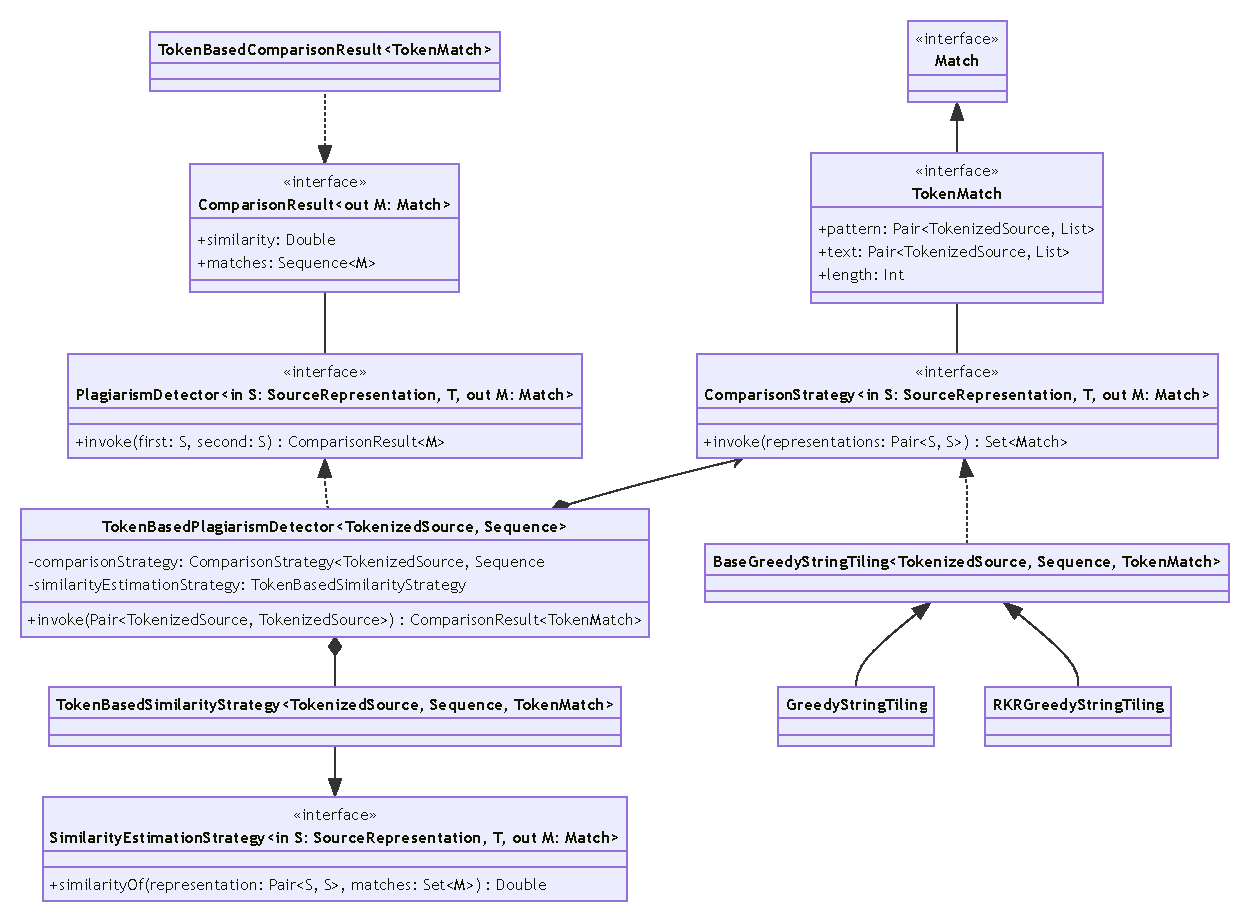
\includegraphics[width=\textwidth]{resources/img/02-detector.pdf}
    \caption{Schema UML del \textit{detector}.}
    \label{img:02-detector}
\end{figure}
